\documentclass[acmtog, authorversion]{acmart}

\settopmatter{printacmref=false} % Removes citation information below abstract
\renewcommand\footnotetextcopyrightpermission[1]{} % removes footnote with conference information in first column
\pagestyle{plain} % removes running headers
\acmDOI{} 
\setcopyright{none}

\usepackage{booktabs} % For formal tables

% TOG prefers author-name bib system with square brackets
\citestyle{acmauthoryear}
\setcitestyle{square}

\usepackage[ruled]{algorithm2e} % For algorithms
\usepackage{enumitem}
\usepackage{siunitx}
\usepackage{amsfonts}
\usepackage{amsmath}
\usepackage{bigints}
\usepackage{textcomp}

\renewcommand{\algorithmcfname}{ALGORITHM}
\SetAlFnt{\small}
\SetAlCapFnt{\small}
\SetAlCapNameFnt{\small}
\SetAlCapHSkip{0pt}
\IncMargin{-\parindent}

% Metadata Information
% \acmJournal{TOMS} % {TOG}https://www.overleaf.com/6495666636xyhrjfrqtzzc
\acmJournal{} % {TOG}https://www.overleaf.com/6495666636xyhrjfrqtzzc
\acmVolume{X}
\acmNumber{X}
\acmArticle{XX}
\acmYear{2019}
\acmMonth{4}

% Copyright
%\setcopyright{acmcopyright}x
%\setcopyright{acmlicensed}
%\setcopyright{rightsretained}x
%\setcopyright{usgov}
\setcopyright{usgovmixed}
%\setcopyright{cagov}
%\setcopyright{cagovmixed}

% DOI
\acmDOI{0000001.0000001_2}

% Paper history
\received{May 1, 2019}
\received{Month 2019}
\received[final version]{Month 2019}
\received[accepted]{Month 2019}

%%%%%%%%%%%%%%%%%%%%%%%%%%%%%%%%%%%%%%%%%%%%%%
%%%%%%%%%%%%%%%%%%%%%%%%%%%%%%%%%%%%%%%%%%%%%%
%%%%%%%%%%%%%%%%%%%%%%%%%%%%%%%%%%%%%%%%%%%%%%
\newcommand{\norm}[1]{\lVert #1\rVert}
\newcommand{\R}{\mathbb{R}}
\newcommand{\bvec}[1]{\boldsymbol{#1}}
\newcommand{\vt}{\bvec{t}}
\newcommand{\E}{\mathrm{e}}
\newcommand{\dif}{\mathrm{d}}
\newcommand{\vx}{\bvec{x}}
\DeclareMathOperator*{\argmax}{arg\,max}
\DeclareMathOperator*{\argmin}{arg\,min}

\newcommand{\jhnote}[1]{{\textcolor{blue}{FH: #1}}}
\newcommand{\scnote}[1]{{\textcolor{red}{SC: #1}}}
\newcommand{\alnote}[1]{{\textcolor{orange}{JR: #1}}}

% Document starts
\begin{document}

\copyrightyear{2019} 
\acmYear{2019} 
\setcopyright{rightsretained} 
\acmConference[PEARC '19]{Practice and Experience in Advanced Research Computing}{July 28-August 1, 2019}{Chicago, IL, USA}
\acmBooktitle{Practice and Experience in Advanced Research Computing (PEARC '19), July 28-August 1, 2019, Chicago, IL, USA}
\acmDOI{10.1145/3332186.3333261}
\acmISBN{978-1-4503-7227-5/19/07}


\CopyrightYear{2019} 
\setcopyright{rightsretained} 
\conferenceinfo{PEARC '19}{July 28-August 1, 2019, Chicago, IL, USA}\isbn{978-1-4503-7227-5/19/07}
\doi{https://doi.org/10.1145/3332186.3333261}



% Title portion
\title{A Brief Introduction to GAIL ({\sc Guaranteed Automatic Integration Library}) Version 2.3}

\author{Sou-Cheng T.~Choi}
\orcid{0000-0002-4270-7077}
\affiliation{%
  \institution{Illinois Institute of Technology}
  \streetaddress{10 W 32nd St}
  \city{Chicago}
  \state{IL}
  \postcode{60637}
  \country{USA}}
\email{schoi32@iit.edu} 
\author{Jagadeeswaran Rathinavel}
\orcid{0000-0002-4270-7077}
\affiliation{%
  \institution{Illinois Institute of Technology}
  \streetaddress{10 W 32nd St}
  \city{Chicago}
  \state{IL}
  \postcode{60637}
  \country{USA}}
\email{jrathin1@hawk.iit.edu} 
\author{Xin Tong}
\orcid{0000-0002-4270-7077}
\affiliation{%
  \institution{University of Illinois at Chicago}
  \streetaddress{1200 W Harrison St}
  \city{Chicago}
  \state{IL}
  \postcode{60607}
  \country{USA}}
\email{xtong5@hawk.iit.edu} 
\author{Kan Zhang}
\orcid{0000-0002-4270-7077}
\affiliation{%
  \institution{Illinois Institute of Technology}
  \streetaddress{10 W 32nd St}
  \city{Chicago}
  \state{IL}
  \postcode{60637}
  \country{USA}}
\email{kzhang23@hawk.iit.edu} 
\author{Fred J.~Hickernell}
\orcid{0000-0002-4270-7077}
\affiliation{%
  \institution{Illinois Institute of Technology}
  \streetaddress{10 W 32nd St}
  \city{Chicago}
  \state{IL}
  \postcode{60637}
  \country{USA}}
\email{hickernell@iit.edu} 

\renewcommand\shortauthors{Choi, S.-C. T. et al}


\begin{abstract}
Function approximation, optimization, and integration over (in)finite
domains are among the most fundamental mathematical problems. They  are
particularly challenging when the functions in consideration fluctuate
wildly in certain parts of the domain or if the domain is high dimensional.
Development of efficient and effective numerical algorithms for
approximating the solutions to these problems that are based on rigorous
mathematical frameworks, (statistical) error bounds, advanced sampling
strategies, and careful complexity analysis remain active research areas. 
The Guaranteed Automatic Integration Library (GAIL) %~\cite{ChoEtal18b} 
is our multi-year research efforts directed towards addressing the
aforementioned overarching theme. Briefly, GAIL is an open-source MATLAB
software package with eight main algorithms based on over ten peer-reviewed
publications, involving more than nine doctoral students and three faculty
members in Illinois Tech as well as their international collaborators.  The
theories behind our algorithms consider functions in cones, rather than
balls, and then proceed to sample data points of a given function in an
adaptive manner, placing more samples in areas where the function changes
faster. Our algorithms are iterative in nature, with errors bounds computed
in each iteration. They are proven to have optimal costs, with monotonic
decreasing error estimates and stop in the first iteration where user-given
tolerance is met.  We consistently employ proven industrial software
development practices for GAIL such as unit and integration tests,
searchable online and offline documentation, version control systems
(GitHub), and agile methodology (using Trello). Our reproducible research
have demonstrated that GAIL could outperform more established algorithms in
various ways.   
\end{abstract} 


%
% The code below should be generated by the tool at
% http://dl.acm.org/ccs.cfm
% Please copy and paste the code instead of the example below.
%
%
%How To Assign CCS Concepts:
%Browse the CCS by clicking through the desired nodes (subject areas) or scroll through the Flat View
%Click on "Assign This CCS Concept" from the left menu, or on the subject itself in the Flat View, when you have reached the appropriate level of subject granularity
%Choose the proper relevance of the chosen CCS concept (High, Medium, Low)
%The full classification you have chosen so far will display; adjust the relevance of the current node if necessary
%Choose [continue] to find and assign the next CCS Concept
%Once complete, click on "Generate CCS Codes"
%Copy and Paste the appropriately formated CCS Coding to the item you are classifying
%Choose [done] only after you have pasted the information into the item you are classifying
%
%Guidelines For Assigning CCS Concepts:
%Choose as many classifications as you feel appropriate to best convey the subject areas of your item
%The average number of classificaitons per item is three
%It is not recommended to choose more than five
%Each classification chosen must be assigned a relevance based on a three level scale (High 500, Medium 300, Low 100)
%Be sure and choose at least one at the highest relevance (500)
%It is not recommended to assign the highest relevance to more than one CCS concept

\begin{CCSXML}
<ccs2012>
<concept>
<concept_id>10002950.10003648.10003671</concept_id>
<concept_desc>Mathematics of computing~Probabilistic algorithms</concept_desc>
<concept_significance>500</concept_significance>
</concept>
<concept>
<concept_id>10003752.10003809.10003636.10003815</concept_id>
<concept_desc>Theory of computation~Numeric approximation algorithms</concept_desc>
<concept_significance>500</concept_significance>
</concept>
<concept>
<concept_id>10002950.10003705.10011686</concept_id>
<concept_desc>Mathematics of computing~Mathematical software performance</concept_desc>
<concept_significance>500</concept_significance>
</concept>
<concept>
<concept_id>10011007.10011074</concept_id>
<concept_desc>Software and its engineering~Software creation and management</concept_desc>
<concept_significance>300</concept_significance>
</concept>
<concept>
<concept_id>10011007.10011074.10011134</concept_id>
<concept_desc>Software and its engineering~Collaboration in software development</concept_desc>
<concept_significance>300</concept_significance>
</concept>
</ccs2012>
\end{CCSXML}

\ccsdesc[500]{Mathematics of computing~Probabilistic algorithms}
\ccsdesc[500]{Theory of computation~Numeric approximation algorithms}
\ccsdesc[500]{Mathematics of computing~Mathematical software performance}
\ccsdesc[300]{Software and its engineering~Software creation and management}
\ccsdesc[300]{Software and its engineering~Collaboration in software development}
%
% End generated code
%


\keywords{adaptive sampling, function approximation, global optimization, (quasi-)Monte Carlo, cubature, error analysis, stopping criteria}

\maketitle

\section{Introduction}
\label{sec:intro}

 TBD\\
 
\section{Algorithms}
\label{sec:algo}

GAIL's latest release, version 2.3, includes the following algorithms:
\begin{enumerate} [label=\Roman*.]

\item Approximation and optimization:

    \begin{enumerate}[label={[\arabic*]}]
    
    \item \texttt{funappx\_g}: One-dimensional function approximation on bounded interval~\cite{FunappxFunmin}
    
    \item \texttt{funmin\_g}: Global minimum value of univariate function on a closed interval~\cite{FunappxFunmin}
    
    \end{enumerate}

\item Integration:

    \begin{enumerate}[label={[\arabic*]}, start=3, resume*]
    
    \item \texttt{integral\_g}: One-dimensional integration on bounded interval~\cite{ChoEtal18b}
    
    \item \texttt{meanMC\_g}: Monte Carlo (MC) method for estimating mean of a random variable~\cite{meanMCcubMC}
    
    \item \texttt{meanMC\_CLT}: MC method with Central Limit Theorem (CLT) confidence intervals for estimating mean of a random variable \cite{ChoEtal18b}
    
    \item \texttt{cubMC\_g}: MC method for  multiple integration \cite{meanMCcubMC}
    
    \item \texttt{cubSobol\_g}: Quasi-Monte Carlo (QMC) method using Sobol' cubature for multiple integration \cite{cubSobol}
    
    \item \texttt{cubLattice\_g}: QMC method using rank-1 lattices cubature for multiple integration \cite{cubLattice}
    
    \item \texttt{cubBayesLattice\_g}: Bayesian cubature method using lattice sampling for multiple integration \cite{cubBayesLattice}
    
    \end{enumerate}
\item Option Pricing:
\begin{enumerate}\setlength\itemsep{1em}
\item \texttt{assetPath}: A class of discretized stochastic processes that model the values of an asset with respect to time \cite{ChoEtal18b}
\item \texttt{optPayoff}: A class of option payoffs based on asset paths \cite{ChoEtal18b}
\item \texttt{optPrice}: A class that computes the price of an option via (quasi-)Monte Carlo methods \cite{ChoEtal18b}
\end{enumerate}

\end{enumerate}


 
\section{Numerical Examples}
\label{sec:ex}

In this section, we showcase GAIL's performance with two examples on
univariate function optimization and cubature.

\begin{example}\label{eg1} We want to find the global minimum of the following functions: 
\begin{align}
    f(x) &= -5 \E^{-100(x-0.2)^2}-\E^{ -80(x-0.65)^2}  \mbox{ for } x \in [0, 1], \label{eq1}
\\  f(x) &= \sin (10 \pi x^4 ) - x  \mbox{ for } x \in [0, 2]. \label{eq2}
\end{align}
In the case of (\ref{eq1}), \texttt{funmin\_g} automatically samples the
function more often in spiky areas and locates the global minimum
accurately. In contrast, MATLAB's
\texttt{fminbnd}~\cite{brent2013algorithms,forsythe1977computer} returns a
local minimum.  That said, we note that \texttt{fminbnd} was designed for
seeking a local minimum. Chebfun~\cite{TrefEtal17a} approximates $f$ with
Chebyshev polynomials and samples $f$ at Chebyshev points. Its \texttt{min} function is 
capable of returning all local minimum that it
could find, out of which we extract the global minimum. Both \texttt{min} and
\texttt{funmin\_g} succeeded in locating the global minimum to required
accuracy, with the former being more efficient with fewer sampling points
and the latter more accurate.


In the case of (\ref{eq2}), we have a function that is increasingly
oscillating as $x$ increases and the true minimum occurs at the right
boundary point. Both \texttt{min} and \texttt{funmin\_g} were able to return  
accurate approximations, but \texttt{fminbnd} once again settled at a local
minimum far away from the global minimum. The total run time of
\texttt{funmin\_g} was substantially less than that of \texttt{min} because it
sought only the global minimum and disregarded the other local minima.

We plot $f(x)$ and the minima returned by \texttt{funmin\_g}, \texttt{min},
and \texttt{fminbnd}  for the two given functions in Figures~\ref{fig1} and
\ref{fig2}. In addition, Table~\ref{tab1} summarizes the solvers'
performance.

\begin{figure} % MATLAB Driver: min_pearc.m
\centering
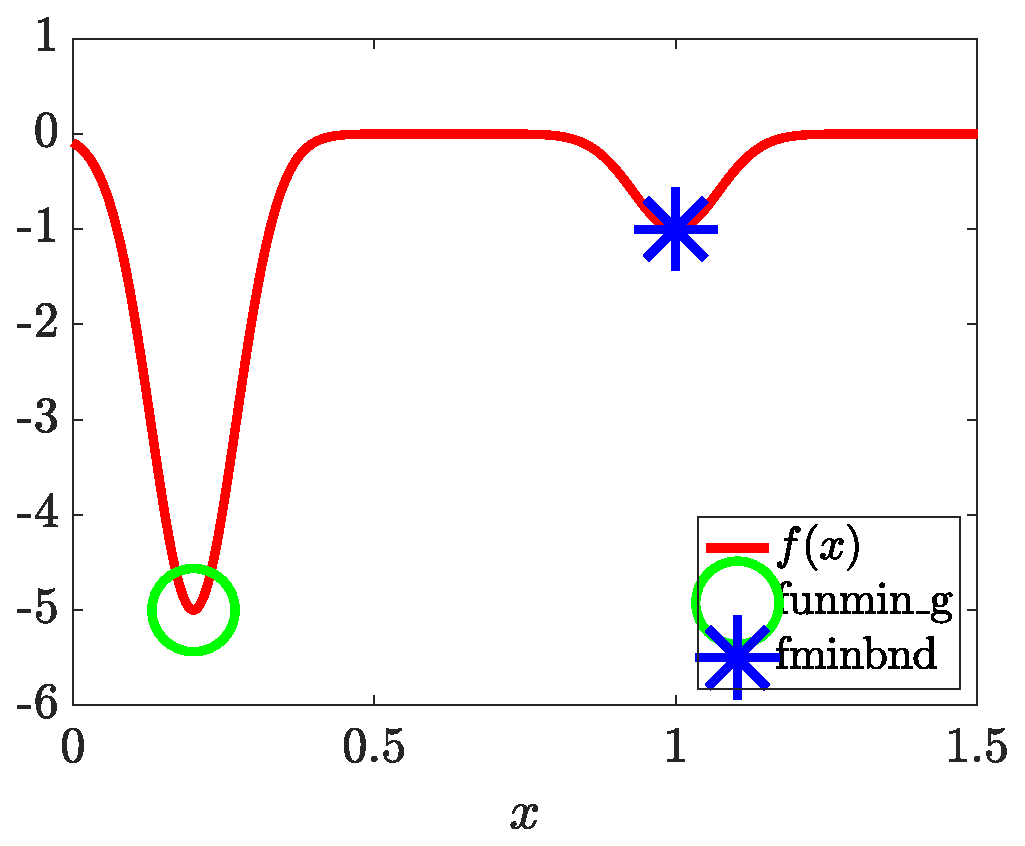
\includegraphics[width = 0.48\textwidth]{humps.eps} 
\caption{We plot the function $f$ in (\ref{eq1}), along with the sampling
points and best estimates of $(x^*, f(x^*)$ from the three solvers,
MATLAB's \texttt{fminbnd}, Chebfun's \texttt{min}, and GAIL's \texttt{funmin\_g}. 
This figure is
reproducible by the MATLAB script, \texttt{min\_pearc.m}, in GAIL.}\label{fig1}
\end{figure}

\begin{figure} % MATLAB Driver: min_pearc.m
\centering
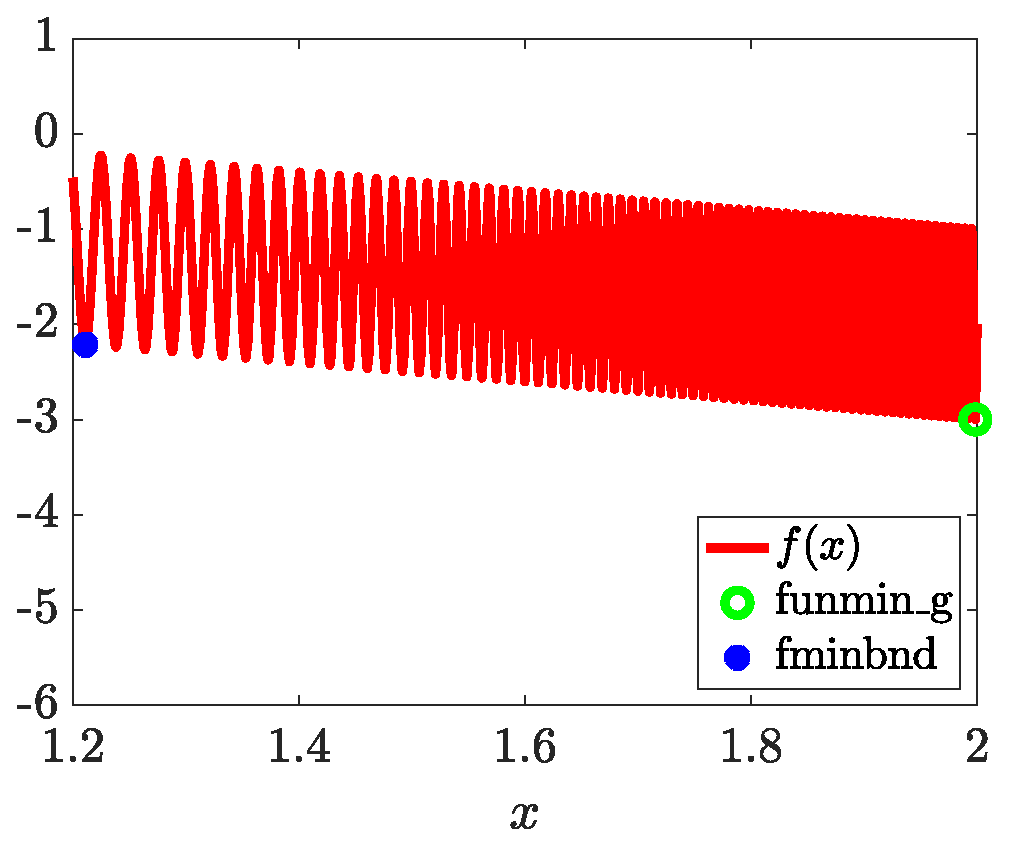
\includegraphics[width = 0.48\textwidth]{sine.eps} 
\caption{
This figure is reproducible by the script, \texttt{min\_pearc.m}, in GAIL.}\label{fig2}
\end{figure}

\begin{table} % MATLAB Driver:  min_pearc.m
\centering
	\caption{Performance of \texttt{funmin\_g}, \texttt{fminbnd}, and
	\texttt{min} with automatic stopping criteria for optimizing
	functions defined in (\ref{eq1}) and (\ref{eq2}). Absolute errors in
	$x$  and $y$ are defined as $|x^* - \hat{x}|$ and $|f(x^* ) -
	f(\hat{x})|$, respectively. These results can be reproduced with script
	\texttt{min\_pearc.m} in GAIL. \label{tab1}}  \vspace{-2ex}
	$
    \begin{array}{l@{\qquad}r@{\quad}r@{\quad}r}
	\input{minPearcOut.txt} 
	\end{array}
	$
\end{table}
\end{example}


\begin{example}\label{eg4}  
In this example, we compare GAIL's Monte Carlo and quasi-Monte Carlo
methods in similar ways as in Section~4 in \cite{hickernellmonte} with the
Keister integrals~\cite{keister1996multidimensional}:
\begin{align}
\mu % & =  \int_{\R^d} \cos(\lVert \vt \rVert_2)  \E^{-\lVert\vt \rVert_2^2} \, \dif \vt \\
& = \bigint_{[0,1]^d} \pi^{d/2} 
\cos \left( \sqrt{ \frac{1}{2} \sum_{j=1}^d \Phi^{-1}(x_j)} \right)  \, \dif \vx. 
\label{kei}
\end{align}

In Table~\ref{tab2}, we summarize the performance of the methods MC, Sobol,
 Lattice, and Bayes---they refer to the GAIL cubatures, \texttt{cubMC\_g},
\texttt{cubLattice\_g}, \texttt{cubSobol\_g},  \texttt{cubBayesLattice\_g},
respectively.
In the case of $d=3$, all four methods succeeded completely meaning the
absolute error is less than given tolerance, i.e., $|\mu - \hat{\mu}| \le
\varepsilon$, where $\hat{\mu}$ is a cubature's approximated value. The
fastest method was \texttt{cubBayesLattice\_g}.
In the case of $d=8$,   \texttt{cubSobol\_g} achieved 100\% success rate
and was the fastest. But \texttt{cubBayesLattice\_g}  was competitive and
had the smallest average absolute error.

\begin{table} % MATLAB Driver: KeisterCubatureExamplePEARC.m
\centering
	\caption{Average performance of cubatures with automatic stopping 
	criteria for estimating the integrals in \eqref{kei}
	for $1000$ independent runs. These results can be conditionally reproduced with the
	script, \texttt{KeisterCubatureExamplePEARC.m}, in GAIL. 
	\label{tab2}}	   \vspace{-2ex}
	$
	%\arraycolsep=1.4pt\def\arraystretch{0.9}
    \begin{array}{l@{\qquad}r@{\quad}r@{\quad}r@{\quad}r@{\quad}r}
	\input{KeisterPearcOut.txt} 
	\end{array}
	$
\end{table}


\end{example} 
\section{Conclusions and Future Work}
\label{sec:concl}
We have presented a short overview of GAIL with some motivating
examples. GAIL and the research behind the software are still under active
development. We list in the following some of the potentially fruitful
directions to pursue in order to strengthen the software.

For the existing algorithms, it would be worthy to conduct or develop
large-scale tests such as work of
~\cite{dolan2002benchmarking,floudas2013handbook} for optimization
problems, to challenge the software for performance in terms of success
rates, execution speed, and memory usage. These test suites could serve to
be a more rigorous basis of comparisons with more established solvers  or
to validate future incremental changes in our own.  

Instead of using \texttt{fminbnd} in Example~\ref{eg1}, it would be better
to use solvers that are designed for global optimization such as those from
 MATLAB's Global Optimization Toolbox (GOT). That said, GOT does not
guarantee returning global minimum; see~\cite{GOT}. Likewise, for 
Example~\ref{eg4}, more extensive study can be done. An
idea is to price Asian options with GAIL cubatures and also
\texttt{asianbyls} from MATLAB's Financial Instruments Toolbox.

We are upgrading Bayesian cubature algorithm to use Sobol' points and Walsh
kernel whereas the current version uses rank-1 lattice points and
shift-invariant kernel. One major advantage is that Walsh kernel based
algorithm does not require the integrand to be periodic, which opens up
more possibilities. Additional improvements being developed are to add
gradient in parameter searching; this will allow using gradient descent
method instead of heuristic search, and could possibly speed up the algorithm.
Shift-invariant kernel used in the algorithm is currently limited to order
of even integers which is usually fixed. Enhancements are being developed
to avoid this constraint.

Each GAIL algorithm could find itself into many high-impact application
areas such as computational finance, machine learning, decision sciences.
Reliable cubatures are particularly important for valuing financial
derivatives. GAIL already contains a few option-pricing functions,  
namely, \texttt{assetPath}, \texttt{optPayoff}, and  \texttt{optPrice}. 
However, they have yet to elevated as a first-class citizens in
the software library, which have to be accompanied by detailed documentation
and unit tests suites.

Currently, most of the GAIL algorithms are written and released in Matlab. Recently other computer languages are getting popular in scientific computing. Given the flexibility of GAIL software design, it could very well be ported or language interface is added to support Python, Julia and R languages.
\begin{comment}
\begin{enumerate}

\item \texttt{assetPath}: A class of discretized stochastic processes that
model the values of an asset with respect to time

\item \texttt{optPayoff}: A class of option payoffs based on asset paths

\item \texttt{optPrice}: A class that computes the price of an option via
(quasi-)Monte Carlo methods.

\end{enumerate}


\alnote{Is there any future to support another popular scientific computing
language? like Julia ? Should we mention Fred's idea to bring other
collaborators? Or mention here interested collaborators contact us at--- ?}
\scnote{QMC Community software and OO classes}
\end{comment}


\begin{acks}
Our work was supported in part by grants from the National
Science Foundation under grants NSF-DMS-1115392 and NSF-DMS-1522687, and the Office
of Advanced Scientific Computing Research, Office of Science,
U.S. Department of Energy, under contract DE-AC02-06CH11357.
  
The authors would like to thank all GAIL contributors,
especially Yuhan Ding, Lan Jiang, Llu\'is Antoni Jim\'enez
Rugama, Aleksei Sorokin, and Yizhi Zhang.
\end{acks}

\bibliographystyle{ACM-Reference-Format} %abbrv
\bibliography{gail_papers}

\end{document}
